\documentclass[11pt,a4paper,twocolumn]{article}

% Fundamental Packets
\usepackage[utf8]{inputenc}         % chars codification
\usepackage[T1]{fontenc}            % font encoding
\usepackage[italian,english]{babel} % multilingual (english default)
\usepackage{amsmath,amssymb}        % maths symbols
\usepackage{graphicx}               % images
\usepackage{booktabs}               % professional tables
\usepackage{geometry}               % margin management
\usepackage{cite}                   % citations
\usepackage{url}                    % urls in bibliography
\usepackage{float}                  % image exactly where placed with [H]
\usepackage{subcaption}
\graphicspath{{./src/}}
% margins
\geometry{left=1.5cm, right=1.5cm, top=1.5cm, bottom=2cm}

% Doc info
\title{Predicting Acute Oral Toxicity ($LD_{50}$): A Machine Learning and Deep Learning Approach using Molecular Descriptors and Graph Representations}
\author{Group 5 Members \\ 
        \small \textit{Abate Luca, Bernacchia Alessia, Pioda Tommaso, Villani Giacomo} \\
        \small \textit{Department of Innovative Technologies} \\
        \small \textit{SUPSI}}
\date{\today}

\begin{document}

\maketitle

\begin{abstract}
Acute toxicity prediction is a cornerstone of drug discovery, as 
toxicity-related failures account for a significant portion of preclinical 
compound attrition. In this project, we utilize the Therapeutics Data Commons 
(TDC) $LD_{50}$ dataset, comprising 7,385 drug molecules, to develop a predictive 
framework. We implement a rigorous data pipeline involving chemical standardization 
and the extraction of hybrid descriptors, including Morgan, Avalon, and ErG 
fingerprints, alongside Dragon-derived physicochemical features. We evaluate 
the performance of classical machine learning models (Random Forest, Ridge, 
SVM, XGBoost) and deep learning architectures (CNN, GNN). Our methodology 
emphasizes data consistency and feature engineering to ensure that the models 
generalize effectively to novel chemical structures, ultimately aiming to 
reduce preclinical attrition and enhance drug safety profiles.
\end{abstract}

\section{Introduction}
The majority of drugs exhibit some degree of toxicity to human organisms. Accurate prediction of these effects is critical, as toxicity is one of the primary causes of compound attrition in the pharmaceutical pipeline. Studies indicate that approximately 70\% of all toxicity-related attrition occurs preclinically, yet these findings are strongly predictive of toxicities in humans. Consequently, early and accurate toxicity prediction can significantly reduce compound attribution and boost the likelihood of a drug successfully reaching the market.

This study focuses on the prediction of the median lethal dose ($LD_{50}$), a standard measure of acute toxicity. A significant challenge in this task is generalization: as drug structures evolve, models must maintain accuracy on novel drugs with low structural similarity to existing datasets. Our project addresses this by combining traditional physicochemical descriptors with advanced molecular fingerprints and graph-based deep learning, ensuring a comprehensive representation of chemical space.

\section{Materials \& Methods}

\subsection{Data Collection}
The dataset was obtained from the Therapeutics Data Commons (TDC) for the Acute Toxicity $LD_{50}$ task \cite{TDC_LD50}. The raw data provides Drug IDs, SMILES strings, and the target toxicity label ($Y$). The dataset consists of 7,385 small molecules, partitioned into the following sets:
\begin{itemize}
    \item \textbf{Training Set}: 5,169 samples (70\%)
    \item \textbf{Validation Set}: 738 samples (10\%)
    \item \textbf{Test Set}: 1,478 samples (20\%)
\end{itemize}

\subsection{Data Cleaning and Consistency}
Rigorous data cleaning was performed to ensure the quality of the inputs. The process involved:
\begin{itemize}
    \item \textbf{Standardization}: SMILES strings were checked for chemical validity using RDKit; 0 invalid strings were found across all sets.
    \item \textbf{Missing Values}: The dataset was confirmed to be complete, with no missing values in any columns.
    \item \textbf{Salt Stripping}: We utilized RDKit's \texttt{SaltRemover} to strip counter-ions and salts, ensuring that descriptors reflect only the parent organic molecule. No salts were detected in the current splits.
    \item \textbf{Duplicate and Inconsistency Handling}: No identical duplicates were found. However, we identified 15, 5, and 10 inconsistent SMILES in the train, valid, and test sets, respectively (where the same molecule was associated with different labels). We chose to retain these cases to represent natural assay variability, documenting them for evaluation.
\end{itemize}

\subsection{Molecular Descriptors and Feature Engineering}
We extracted three types of molecular fingerprints and two sets of physicochemical descriptors to capture diverse chemical properties without including the target $LD_{50}$ in the feature construction:
\begin{itemize}
    \item \textbf{Morgan Fingerprints}: Capture local atom environments via circular pathways.
    \item \textbf{Avalon Fingerprints}: Based on path-based enumeration and feature substructures \cite{Partex}.
    \item \textbf{ErG Fingerprints}: Capture pharmacophore features and topological distances \cite{Partex}.
    \item \textbf{General Descriptors}: Features like Molecular Weight, LogP, and TPSA \cite{Partex}.
    \item \textbf{Dragon Descriptors}: Advanced topological and electronic descriptors extracted based on established QSAR methodologies \cite{QSAR_Paper}.
\end{itemize}

\subsection{Model Selection and Embedded Feature Selection}
We implemented a range of models to compare traditional and deep learning approaches:
\begin{itemize}
    \item \textbf{Machine Learning}: Random Forest, Ridge Regression, Support Vector Machines (SVM), and XGBoost.
    \item \textbf{Deep Learning}: Convolutional Neural Networks (CNN) for sequence/grid data and Graph Neural Networks (GNN) to process molecular graphs directly.
    \item \textbf{Embedded Feature Selection}: To manage high dimensionality, we utilize embedded methods (e.g., Lasso or tree-based importance) that perform selection during training, identifying the most predictive features while reducing noise.
\end{itemize}

\section{Data Exploration and Processing}
% This section includes the details of the steps taken before modeling.
\subsection{Initial Statistics}
The initial dataset imported 7,385 drugs. Distribution analysis of the $LD_{50}$ values was conducted to understand the range of toxicity across the chemical space.

\subsection{Cleaning Results}
As noted in the Methods, the cleaning process verified the integrity of the TDC data. The lack of invalid SMILES and missing values suggests a high-quality initial collection. The removal of salts ensures that descriptors like Molecular Weight are not skewed by irrelevant counter-ions.

\subsection{Basic Data Exploration}
Basic exploratory data analysis confirmed that the processed training, validation, and test partitions contain no missing values, and that the target distributions are consistent across all sets (as shown in Figure~\ref{target_distr}). 
Scaffold analysis showed a high number of unique molecular frameworks and essentially zero overlap between partitions, indicating that the model evaluation is based on scaffold-split generalization rather than memorization of known structures. 
Spearman correlation analysis and a linear regression baseline identified the most predictive descriptors and provided an initial ranking of feature relevance.
In addition through ANOVA analysis we were able to extrapolate the most significant features that are shown in Figure~\ref{anova}

\begin{figure}[H] %here in the text
    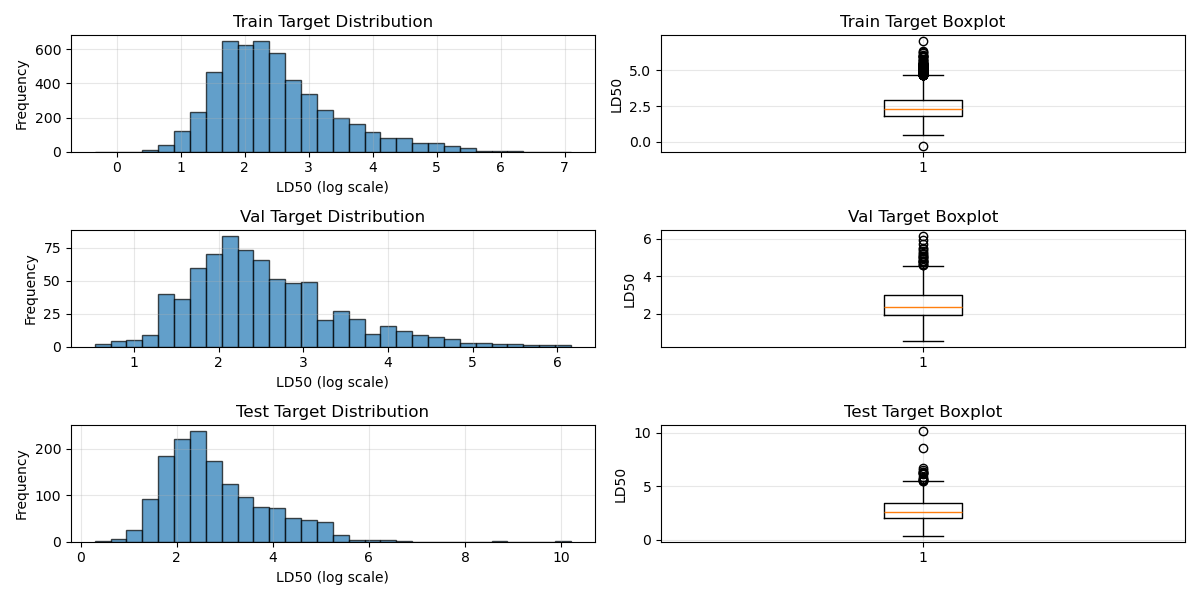
\includegraphics[width=\linewidth]{exploration/target_distribution.png}
    \caption{Comparison of sets' target distribution.}
    \label{target_distr}
\end{figure}

\begin{figure}[H] %here in the text
    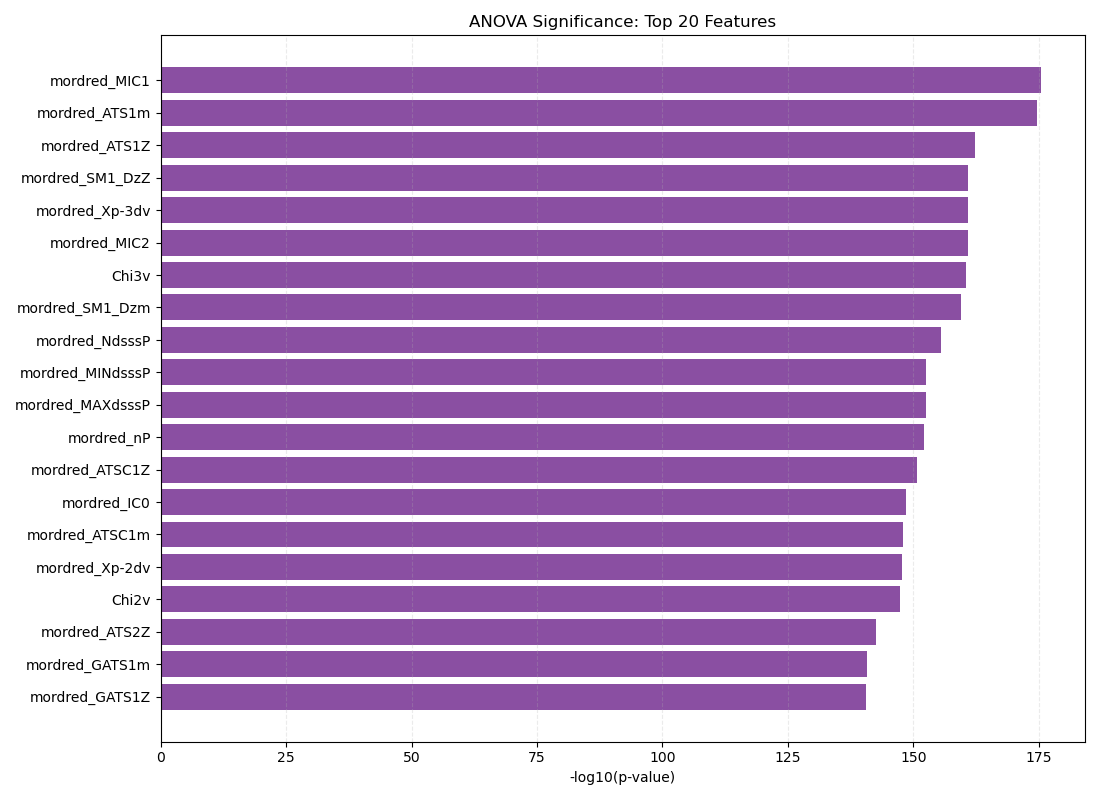
\includegraphics[width=\linewidth]{exploration/anova.png}
    \caption{ANOVA significant features $p < 0.05$.}
    \label{anova}
\end{figure}

\subsection{Advanced Data Exploration}
Advanced analysis investigated descriptor-level variability, outliers, and the intrinsic dimensionality of the feature space. 
Outliers were detected using both IQR and Z-score thresholds (as shown in Figure~\ref{outliers}), and feature dispersion was measured using the coefficient of variation (as shown in Figure~\ref{coeff_var}). 
Principal Component Analysis (PCA) with robust scaling quantified the number of components required to capture the majority of variance, while multi-scale PCA projections revealed structure in the chemical-toxicity relationships showed in Figure~\ref{pca_multiscale}. 
Finally, ANOVA across discretized low, medium, and high toxicity groups identified descriptors with statistically significant differences, highlighting promising features for downstream modeling.
\begin{figure}[H] %here in the text
    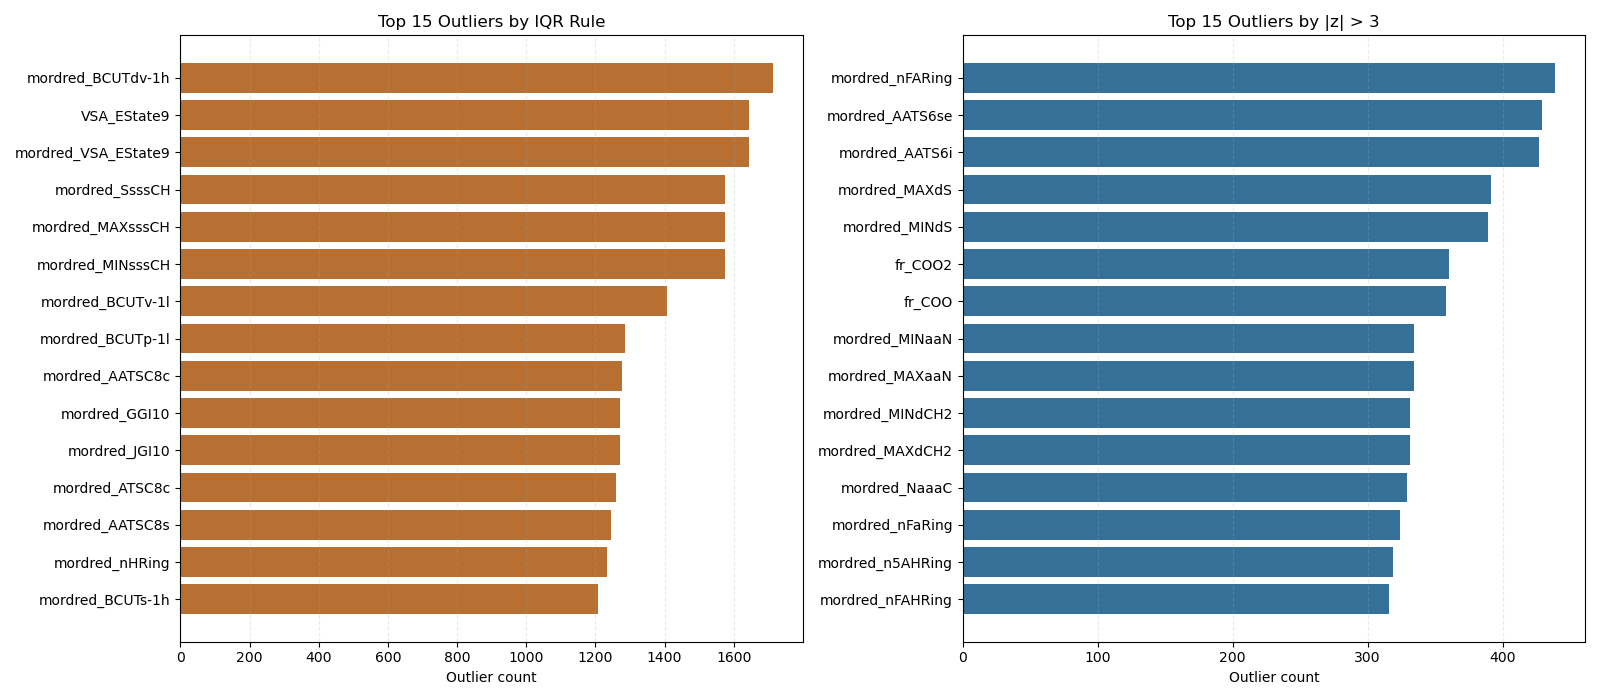
\includegraphics[width=\linewidth]{exploration/top_features_outliers.png}
    \caption{Set of the top features with outliers.}
    \label{outliers}
\end{figure}

\begin{figure}[H] %here in the text
    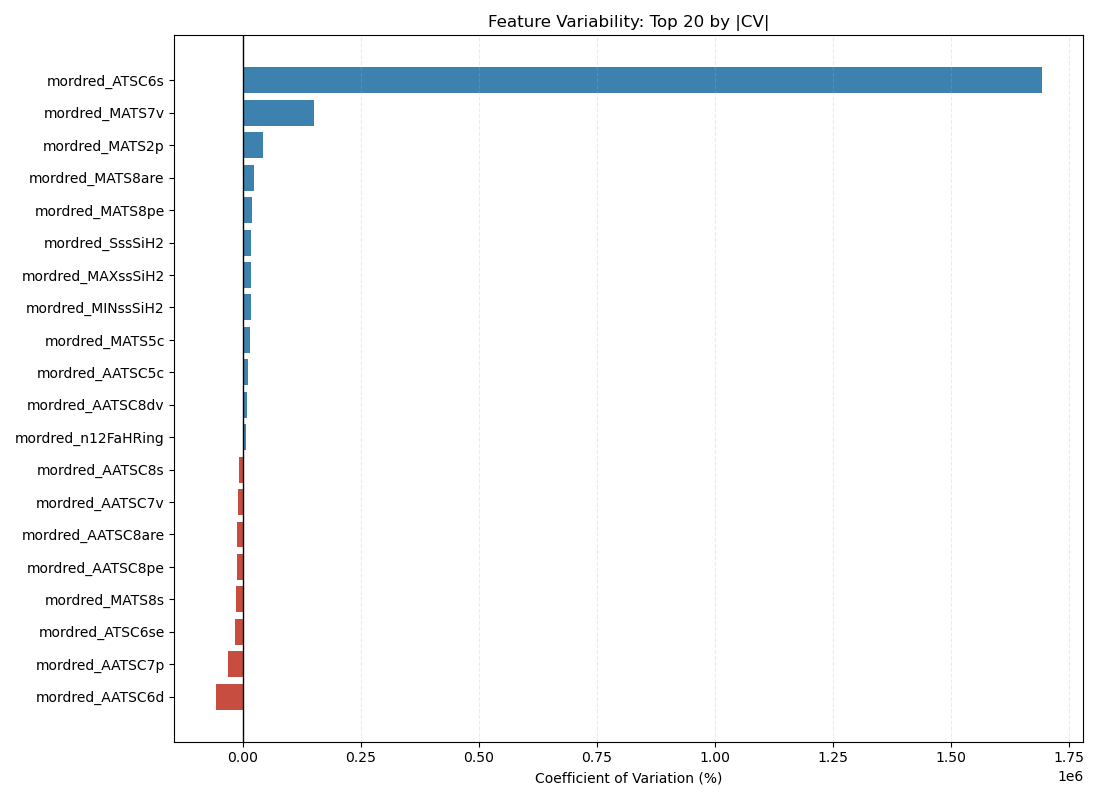
\includegraphics[width=\linewidth]{exploration/features_coefficient_variation.png}
    \caption{Coefficient of variation.}
    \label{coeff_var}
\end{figure}

\begin{figure}[H] %here in the text
    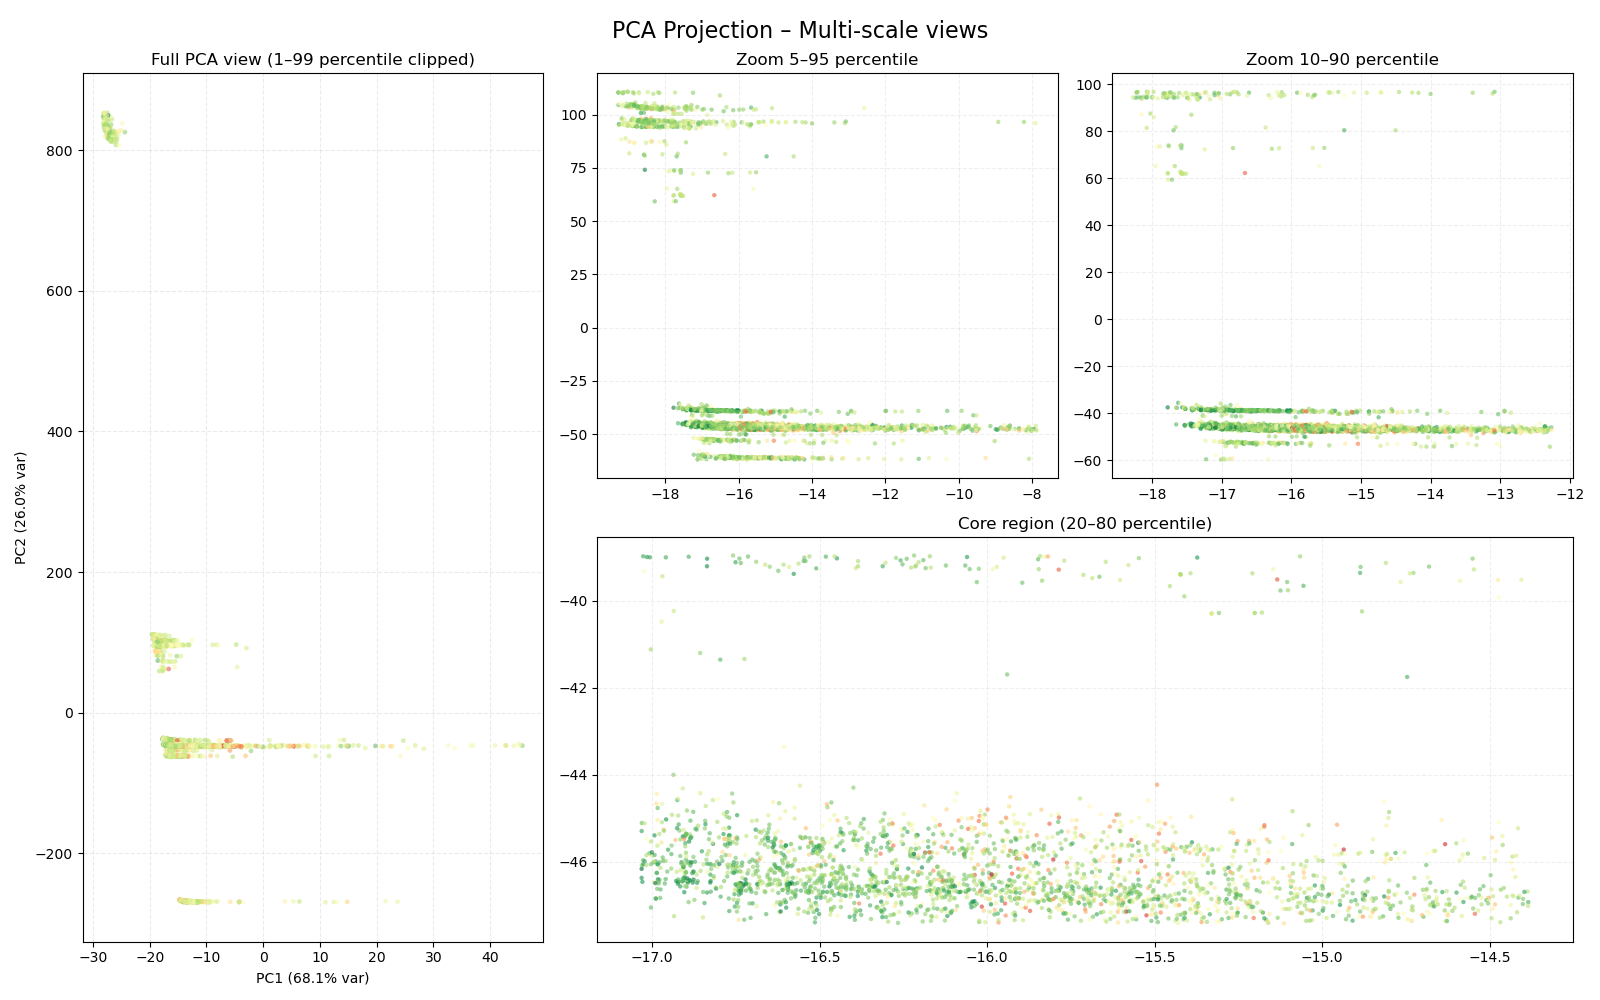
\includegraphics[width=\linewidth]{exploration/PCA_multiscale.png}
    \caption{PCA with multiple scale representation.}
    \label{pca_multiscale}
\end{figure}

\subsection{Feature Selection}
Given the high dimensionality of the initial dataset (1,816 features), a rigorous feature selection procedure was implemented. This process aims to mitigate the risk of overfitting, enhance model performance, and optimize computational efficiency by retaining only the most informative descriptors for predicting $LD_{50}$.
Our feature selection pipeline is structured as follows:

\begin{itemize}
    \item \textbf{Spearman Filter}: This step removes redundant features by identifying highly collinear pairs and filtering those with weak monotonic relationships to the target $LD_{50}$, ensuring a lean and non-redundant input space.
    \item \textbf{Random Forest Regressor}: We leverage tree-based Mean Decrease in Impurity (MDI) to rank features. This allows us to identify descriptors with significant non-linear predictive power and structural importance.
    \item \textbf{LASSO Feature Importance}: By utilizing $L_1$ regularization, we perform embedded selection. This technique shrinks the coefficients of non-essential descriptors to zero, isolating a sparse yet high-impact feature set.
    \item \textbf{Performance Evaluation}: We systematically monitor the stability and predictive accuracy of the models as the feature count is reduced. This ensures that the truncation of the feature space does not result in the loss of critical chemical information.
    \item \textbf{Permutation Feature Importance}: As a final validation, we measure the increase in prediction error when a feature's values are randomly shuffled. This identifies the true drivers of the model's logic and confirms the reliability of the selected descriptors.
\end{itemize}
The integration of these methods—combining statistical filters, embedded regularization, and post-hoc validation—ensures that the final model is both performant and chemically interpretable.
\clearpage
\begin{figure*}[htbp] % * is to ignore the columns
    \centering
    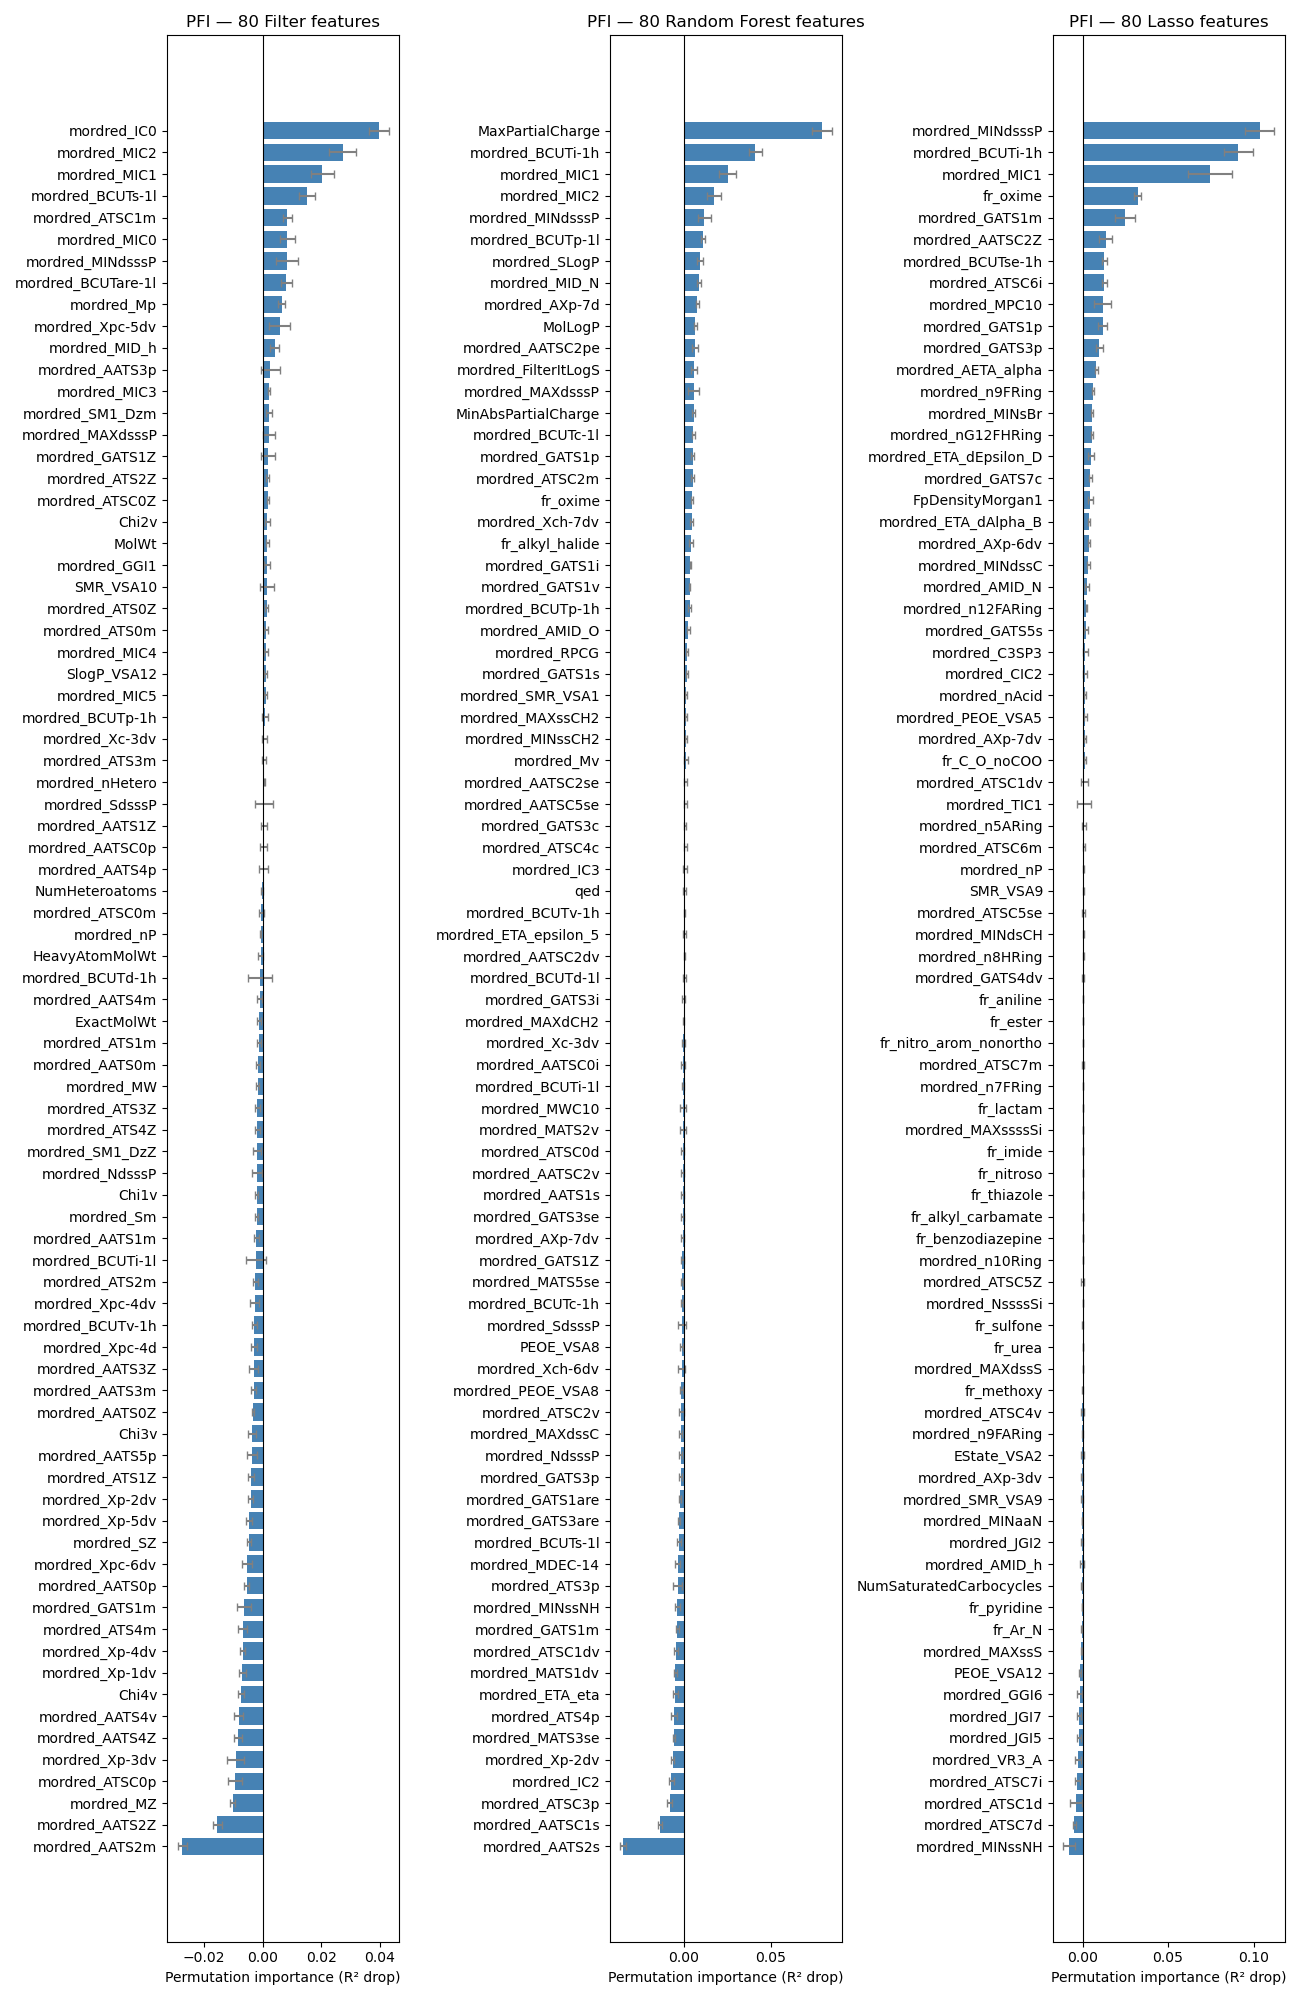
\includegraphics[width=0.9\textwidth]{feat_selection/pfi_comparison.png}
    \caption{Comparison of feature selection techniques.}
    \label{fig:fs_comp}
\end{figure*}
\clearpage


\subsection{Inconsistency Rationale}
The identified inconsistent samples (30 in total) were maintained to prevent the loss of experimental variability. In biological assays, $LD_{50}$ values can vary depending on conditions, and keeping these entries allows the models to potentially learn a more robust, averaged representation.

\subsection{Feature Integration}
By combining fingerprints (Avalon, Morgan, ErG) with Dragon descriptors, we create a hybrid feature space. These features are strictly structural and physicochemical, ensuring that no target leakage occurs during the learning process.

\section{Results}
We tested different ML-models to predict the $LD_{50}$ values of the test set. 
The performance metrics used for evaluation are Root Mean Square Error (RMSE), 
Mean Absolute Error (MAE), and Coefficient of Determination ($R^2$).

\begin{table}[H]
\centering
\caption{Performances of the different machine learning models we tried. 
Only test set is considered.}
\label{tab:model_test_comparison}
\footnotesize
\begin{tabular}{@{}lccc@{}}
\toprule
Model & RMSE & MAE & $R^2$ \\
\midrule
Ridge Regression & 1.1126 & 0.7460 & -0.1046 \\
SVM & 0.9336 & 0.6507 & 0.2221 \\
Random Forest & 0.8888 & 0.6289 & 0.2951 \\
Weighted Ensemble & 0.8978 & 0.6269 & 0.2807 \\
\textbf{XGBoost} & \textbf{0.8773} & \textbf{0.6158} & \textbf{0.3132} \\
\bottomrule
\end{tabular}

\vspace{0.6em}
\raggedright
\textbf{Interpretation.}
XGBoost is the best performing model on the test set, since we obtained the 
lowest RMSE and MAE and the highest $R^2$ from it. This result is justified 
by the nature of the descriptor space: the relationship between molecular 
descriptors and $LD_{50}$ is non linear, sparse, and affected by interactions 
among physicochemical and structural features. Ridge Regression performs poorly
due to its linear nature, while SVM and Random Forest improve the 
fit but remain less effective on the scaffold-split test compounds. 
The weighted ensemble is competitive, especially in MAE, but it does not surpass 
XGBoost, suggesting that the validation-optimized combination adds robustness 
without improving the final held-out ranking.
\end{table}

\section{Discussion \& Conclusion}
The results obtained for Group 5 indicate a toxicity class of [Class Number] according to the GHS (Globally Harmonized System). Comparing these results with historical data suggests that [Your Conclusion]. 

In conclusion, while $LD_{50}$ provides a fundamental baseline for toxicity, modern toxicology is increasingly moving towards alternative methods (3Rs: Replacement, Reduction, Refinement) to minimize animal testing while maintaining high safety standards.

\begin{thebibliography}{99}

\bibitem{TDC_LD50} 
Therapeutics Data Commons. \textit{Acute Toxicity LD50}. 
\url{https://tdcommons.ai/single_pred_tasks/tox/#acute-toxicity-ld50}

\bibitem{Partex} 
Partex ADMETrix. \textit{Advancing ADMET Prediction: A Hybrid Machine Learning Framework}. 
\url{https://github.com/partex-nv-opensource/tdc-submission/blob/main/src/ics-admet-prediction-tdc-versiontwo/report/Advancing%20ADMET%20Prediction_%20A%20Hybrid%20Machine%20Learning%20Framework%20(Partex%20ADMETrix).pdf}

\bibitem{QSAR_Paper} 
Zhu et al. \textit{Quantitative Structure-Activity Relationship Modeling of Rat Acute Toxicity by Oral Exposure}. 
\url{https://pubs.acs.org/doi/abs/10.1021/tx900189p}

\bibitem{OCE_Paper}
Huang et al. \textit{A Unified System for Molecular Property Predictions: Oloren ChemEngine and its Applications}. ChemRxiv, 2022.
\url{https://doi.org/10.26434/chemrxiv-2022-zz776}

\end{thebibliography}

\end{document}
